\documentclass[11pt,aspectratio=169,usenames,dvipsnames]{beamer}
\usetheme{SimplePlus}

\usepackage{threeparttable}
\usepackage{booktabs}
\usepackage{xcolor} % For custom colors
\usepackage{tikz} % For styling enumerate numbers
\usepackage{tcolorbox} % For colored box styling
\usepackage{amsmath, amsfonts, amssymb, amsthm} % Math related
\usepackage{natbib}
\usepackage{fontspec}
\usepackage{luatexja}
\usepackage[mathscr]{euscript}

% ---------------- %
% color definition %
% ---------------- %
\definecolor{main}{HTML}{23373B}
\definecolor{pink}{RGB}{180, 50, 110}
\definecolor{orange}{HTML}{FF8000}
\definecolor{red}{HTML}{990000}
\definecolor{blue}{HTML}{004C99}
\definecolor{lightgray}{HTML}{E7E7E7}
\definecolor{gray}{RGB}{90, 90, 90}

\newcommand{\pink}[1]{\textcolor{pink}{#1}}
\newcommand{\orange}[1]{\textcolor{orange}{#1}}
\newcommand{\red}[1]{\textcolor{red}{#1}}
\newcommand{\blue}[1]{\textcolor{blue}{#1}}
\newcommand{\green}[1]{\textcolor{OliveGreen}{#1}}
\newcommand{\magenta}[1]{\textcolor{magenta}{#1}}
\newcommand{\gray}[1]{\textcolor{gray}{#1}}
\newcommand{\purple}[1]{\textcolor{purple}{#1}}
\definecolor{yellow}{HTML}{EDB120}

% \setbeamercolor{alerted text}{fg=blue}

%%% automatically add spaces into enumerate and itemize environment
\let\tempone\itemize
\let\temptwo\enditemize
\renewenvironment{itemize}{\tempone\addtolength{\itemsep}{\fill}}{\temptwo}
\let\tempa\enumerate
\let\tempb\endenumerate
\renewenvironment{enumerate}{\tempa\addtolength{\itemsep}{\fill}}{\tempb}

\usepackage{fontawesome5}
\setbeamertemplate{itemize item}{\faAngleRight}
\setbeamertemplate{itemize subitem}{\faAngleDoubleRight}

\setmainfont{Crimson Pro Light}[
  ItalicFont={* Italic},
  BoldFont={Crimson Pro Medium},
  BoldItalicFont={Crimson Pro Medium Italic}]
\setsansfont{Crimson Pro Light}[
  ItalicFont={* Italic},
  BoldFont={Crimson Pro Medium},
  BoldItalicFont={Crimson Pro Medium Italic}]

\usepackage[mode=tex]{standalone}
\usepackage{tikz}
\usetikzlibrary{decorations}
\usetikzlibrary{decorations.pathreplacing, intersections}
\usepackage{pgfplots}
\usetikzlibrary{calc,positioning}
\usepgfplotslibrary{fillbetween}
\pgfplotsset{compat=newest, scale only axis, width = 10cm}

% --------------------------- %
% Section title page with toc %
% --------------------------- %
\setbeamertemplate{subsection page}{%
    \usebeamertemplate*{section page}
}
\setbeamertemplate{section in toc}[square]
\setbeamertemplate{subsection in toc}[square]
\AtBeginSection[]{
% \sepframe
\begin{frame}[noframenumbering]{Outline}
    % \tableofcontents[currentsection]
    \tableofcontents[currentsection, currentsubsection]
\end{frame}
}
\AtBeginSubsection[]{
  \begin{frame}[noframenumbering]{Outline}
    \tableofcontents[currentsection, currentsubsection]
  \end{frame}
}

% ------------ %
% beamerbutton %
% ------------ %
\newcommand{\goto}[2]{\hyperlink{#2}{\beamergotobutton{#1}}}
\newcommand{\return}[2]{\hyperlink{#2}{\beamerreturnbutton{#1}}}
\newcommand{\extgoto}[2]{\href{#2}{\beamergotobutton{#1}}}

\hypersetup{
    pdfpagemode=UseNone,
    pdftitle = {Macroeconomics I, Lecture 9},
    pdfauthor = {Hui-Jun Chen},
    pdfsubject = {},
    pdfkeywords = {},
}

\title[Lecture 9]{Lecture 9 \\ Social Planner's Problem}
\author[Hui-Jun Chen]{Hui-Jun Chen}
\institute[NTHU]{National Tsing Hua University}
\date{\today}

\begin{document}

% Title Page
\begin{frame}[plain]
    \titlepage
\end{frame}

\begin{frame}{Overview}
\label{slide:Overview}
    After constructing both \alert{consumers'} and \alert{firms'} problem, we start to bring them together in \alert{one-period model}:
    \begin{itemize}
        \item Lecture 8: \alert{competitive equilibrium} (CE)
        \begin{itemize}
            \item each agent solve their problems individually
            \item aggregate decision determines ``prices'' (wage, rent, etc.)
        \end{itemize}
        \item Lecture 9: \alert{social planer's problem} (SPP)
        \begin{itemize}
            \item imaginary and benevolent social planner determines the allocation
            \item should be the most efficient outcome
        \end{itemize}
        \item Lecture 10: CE and SPP examples
    \end{itemize}
\end{frame}

\begin{frame}{What is Social Planner?}
\label{slide:What_is_Social_Planner_}
\begin{itemize}
    \item \alert{Benevolent dictator} whose goal is to maximize \alert{social welfare} given \alert{technological constraint}
    \item \textbf{Social welfare}: joint ``happiness'' of every agent in this economy
    \begin{itemize}
        \item \alert{consumer}: tangency between IC and budget line in $ ( C, l ) $-plane
        \item \alert{firm}: $ Y = z F( K, N ) = z F( K, h-l ) $
        \begin{itemize}
            \item labor market clearing: $ N = N^{s} = N^{d} $
            \item consistent with consumer behavior: $ N = h - l $
        \end{itemize}
        \item \alert{government}: income-expenditure identity, $ C = Y - G $
        \begin{itemize}
            \item government is not necessary the social planner! (also one of the agents)
        \end{itemize}
    \end{itemize}
    \item \textbf{Technological constraint}: production possibility frontier
\end{itemize}
\end{frame}

\section{PPF}
\label{sec:PPF}

\begin{frame}{Production Possibility Frontier (PPF)}
\label{slide:Production_Possibility_Frontier__PPF_}
    \begin{itemize}
        \item \textbf{Def}: technological possibilities for the whole economy
        %
        \begin{equation}
        \label{eq:PPF}
            C = z F( K, h-l ) - G
        \end{equation}
        %
        \item \textbf{Marginal rate of transformation} (MRT): rate to transform leisure to consumption (through work)
        %
        \begin{equation}
        \label{eq:MRT}
            \begin{split}
                MRT_{l, C}
                    & = z D_{N} F( K, N )
                \\
                    & = MPN
                \\
            \end{split}
        \end{equation}
        %
    \end{itemize}
\end{frame}

\begin{frame}{Production Possibility Frontier (Figure)}
\label{slide:Production_Possibility_Frontier__Figure_}
        \begin{figure}
            \caption{\scriptsize The Production Function and the Production Possibilities Frontier}
            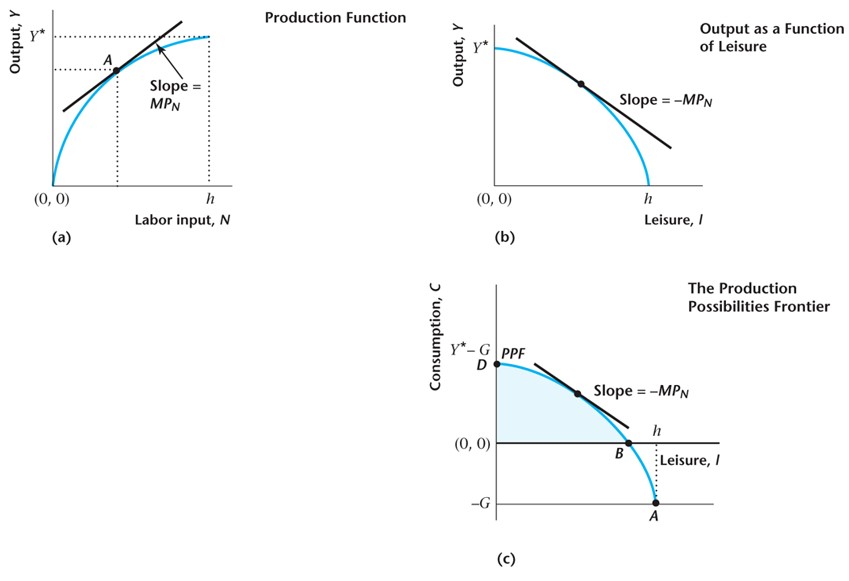
\includegraphics[width=.7\textwidth]{./figures/Figure5_2.jpg}
        \end{figure}
\end{frame}


\begin{frame}{Competitive Equilibrium: Graphcial Representation}
\label{slide:Competitive_Equilibrium__Graphcial_Representation}
    \begin{columns}
        \begin{column}{0.5\textwidth}
            \begin{figure}
                \caption{\scriptsize Competitive Equilibrium}
                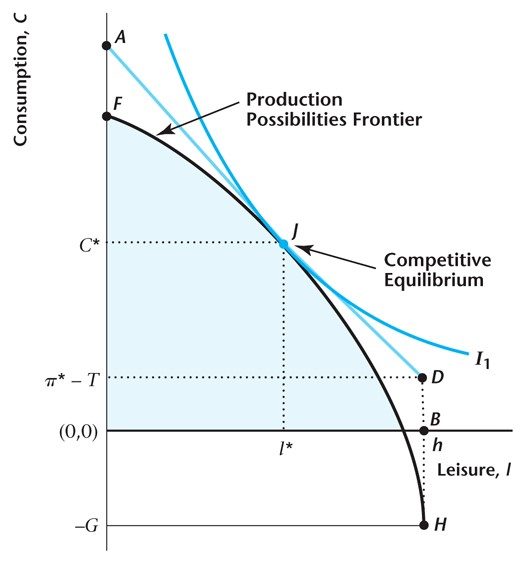
\includegraphics[width=.8\textwidth]{./figures/Figure5_3.jpg}
            \end{figure}
        \end{column}
        \begin{column}{0.5\textwidth}
            Combine PPF with IC:
            \begin{itemize}
                \item $\overline{AD}$: tangent to consumer's IC $ I_{1} $ and PPF $\overline{FH}$
                \item negative slope of $\overline{AD}$: equilibrium wage $ w $
                \begin{itemize}
                    \item $ \because \overline{AD}$ is budget line
                \end{itemize}
                \item Recall Lecture 8 \& last slide:
                \begin{itemize}
                    \item conumser: $ MRS_{l, C} = w $
                    \item firm: $ MPN = w $
                    \item efficiency: $ MRT_{l, C} = MPN $
                \end{itemize}
                %
                \begin{equation*}
                   MRS_{l, C} = MRT_{l, C} = MPN
                \end{equation*}
                %
            \end{itemize}
        \end{column}
    \end{columns}
\end{frame}

\section{Pareto Efficiency}
\label{sec:Pareto_Efficiency}

\begin{frame}{Concept: Pareto Improvement / Optimal}
\label{slide:Concept__Pareto_Improvement___Optimal}
    A competitive equilibrium is \textbf{Pareto optimal} or \textbf{Pareto efficient} if there is no way to \alert{rearrange production or to reallocate goods} so that \alert{someone is made better off} \red{without making someone else worse off}.
    \begin{itemize}
        \item only one consumer, so relatively straightforward
        \item but, still a powerful concept:
        \begin{itemize}
            \item free markets can produce socially efficient outcomes
            \item often easier to analyze social optimum than competitive equilibrium
        \end{itemize}
        \item caveats:
        \begin{itemize}
            \item ``efficiency'' in economics is a statement about a model
            \item very narrow: e.g. having Jeff Bezos pay for a meal for someone in need is ``harming'' Bezos.
        \end{itemize}
    \end{itemize}
\end{frame}

\section{Social Planner}
\label{sec:Social_Planner_s_Problem}

\begin{frame}{Social Planner's Problem}
\label{slide:Social_Planner_s_Problem}
    %
    \begin{align*}
        \text{objective: consumer's utility } \quad
            & \max_{C, l, N, Y} U( C, l )
        \\
        \text{subject to} \quad
            &
        \\
        \text{agg. resource constraint} \quad
            &  C + G \le Y
        \\
        \text{production constraint} \quad
            & Y = z F( K, N )
        \\
        \text{labor constraint} \quad
            & N = h - l
    \end{align*}
    %
    \begin{itemize}
        \item \alert{What's here}: GDP accounting, physical / technological constraints, required government spending, consumer preferences
        \item \alert{What's not}: consumer's budget constraint, the wage rate, consumer's / firm's individual problems, profits, taxes
    \end{itemize}
\end{frame}

\begin{frame}{Solving Social Planner's Problem}
\label{slide:Solving_Social_Planner_s_Problem}
    We know all constraints bind, so by substituting:
    %
    \begin{equation}
    \label{eq:SPPSolve}
        \max_{l} U( z F( K, h-l ) - G, l )
    \end{equation}
    %
    \textbf{FOC}:
    %
    \begin{equation}
    \label{eq:SPPFOC}
        \begin{split}
                & D_{l} U( z F( K, h-l ) - G, l)
            \\
               = &  D_{C}U( z F( K, h-l ) - G, l ) ( z D_{N} F( K, h-l ) )
            \\
        \end{split}
    \end{equation}
    %
    \textbf{Rearrange}:
    %
    \begin{equation}
    \label{eq:SPPRearrange}
        \frac{D_{l} U( z F( K, h-l ) - G, l)}{D_{C}U( z F( K, h-l ) - G, l )} = z D_{N} F( K, h-l ) \Rightarrow MRS_{l, C}  = MRT_{l, C}
    \end{equation}
    %
    Same Result! Why?
\end{frame}

\begin{frame}{Welfare Theorem}
\label{slide:Welfare_Theorem}
    \begin{itemize}
        \item \textbf{First welfare theorem}: under \href{https://en.wikipedia.org/wiki/Fundamental_theorems_of_welfare_economics}{\underline{\alert{certain conditions}}}, the allocation under a competitive equilibrium is Pareto optimal
        \item \textbf{Second welfare theorem}: under \href{https://en.wikipedia.org/wiki/Fundamental_theorems_of_welfare_economics}{\underline{\alert{certain conditions}}}, a Pareto optimal allocation is the allocation for a competitive equilibrium.
        \item straightforward to show here (we already have!), but not always so as conditions not always met!
        \item SPP and CE often alike if not identical, serves as a good benchmark
    \end{itemize}
\end{frame}

\begin{frame}{Social Planner's Problem: Graphical Representation}
\label{slide:Social_Planner_s_Problem__Graphical_Representation}
    \begin{columns}
        \begin{column}{0.5\textwidth}
            \begin{figure}
                \caption{\scriptsize Pareto Optimality}
                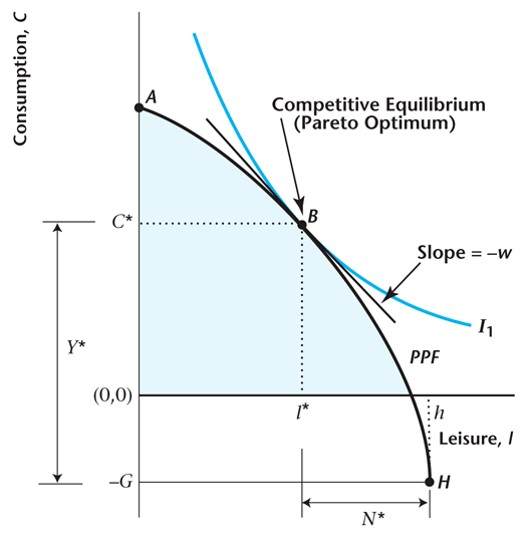
\includegraphics[width=.8\textwidth]{./figures/Figure5_4.jpg}
            \end{figure}
        \end{column}
        \begin{column}{0.5\textwidth}
            Apply SPP \& 2nd welfare theorme for competitive equilibrium:
            \begin{itemize}
                \item $ l^{*} $ determined by SPP at $ B $
                \item $ C^{*}, N^{*}, Y^{*} $ by plugging into constraints
                \item $ w^{*} = MPN = MRT_{l, C} = MRS_{l, C} $
            \end{itemize}
        \end{column}
    \end{columns}
\end{frame}

\begin{frame}{What Can Go Wrong? Cases when SPP $ \neq $ CE}
\label{slide:What_Can_Go_Wrong__Cases_when_SPP____neq___CE}
\begin{enumerate}
    \item Externalities: activity for which an individual does not take account of all associated costs and benefits: can be positive or negative
    \begin{itemize}
        \item example: pollution must be cleaned up, but firm doesn't have to
    \end{itemize}
    \item Distorting taxes: lead to ``wedges'' between MRS, MP, and MRT
    \begin{itemize}
        \item example: proportional labor income tax vs lump-sum tax
    \end{itemize}
    \item Non-competitive / monopolistic behavior: firms or consumers may not be price takers
    \begin{itemize}
        \item examples: local media markets, negotiations
    \end{itemize}
\end{enumerate}
\end{frame}
\end{document}
